\chapter{本项目的创新点}

我在本课题研究中主要是运用了多模态融合、模型优化、跨场景轨迹关联等三项技术创新,在一定程度上解决了传统多目标跟踪在复杂交通场景下不稳定,易断裂的问题,经过仿真实验加实际测试验证证明此算法是可行的,为智慧交通系统的工程应用提供重复使用的方法。以下是详细内容:



\section{多模态传感器融合策略的创新应用}

这篇文章拟从技术革新、应用场景拓展、跨领域交叉这三个方面来进行深入研究。技术创新,我将尝试利用多模态信息、优化深度学习模型和加入强化学习。应用场景拓展,要面对更复杂的应用场景,并与其它交通管理系统紧密合作。跨领域交叉,则主要是多领域的协同工作。相信通过这些措施,多目标跟踪技术能为智慧交通发挥更大的作用,让我们的出行更智能、便捷,发挥重要的技术支持作用。


\subsection{数据融合技术}

我提出激光雷达与摄像头数据对象级融合方案,结合激光雷达点云的三维空间坐标及摄像头二维视觉信息以应对复杂交通场景的目标遮挡、断点等问题。

CARLA仿真平台下,多源传感器同步采样及时空同步使得不同数据精确对齐,大幅提升了目标识别的鲁棒性(如跟踪稳定性提升 16\%)。

\subsection{跨模态特征互补}

用激光雷达的精确的测距能力解决摄像头低照度、复杂的遮挡等问题下的检测盲点, 并以摄像头的外貌特征为对象进行 Re-ID 提供可视信息,完成“探测-跟踪-ReID”的封闭环。



\section{检测跟踪模型的优化与性能突破}

\subsection{模型结构与参数优化}

面向 Town10 复杂交通环境,对已有检测跟踪模型(如 DeepSORT、YOLOv4)进行 架构改进,借助轻量型网络结构(如 MobileNet 主干网络)及多尺度融合等方式,在保 持实时性的前提下,实现跟踪准确率、稳定性与计算速度等至少 3 项核心指标超越 Baseline5\%以上。

加入时空间关联模型,利用 GNN 图神经网络对多个路口车辆间进行建模交互,ID切换率降至 3.2 次 / 分钟,加强了跨路口跟踪连续性。

\subsection{强化学习与元学习结合}

建立元强化学习的自适应优化体系,达到交通流预测与信号控制联合优化如图\ref{fig:p44},实际路测路口通过能力提高22\%,为ITS 动态决策提供了新思路。


\begin{figure}[htbp] % 可以是h(here),t(top),b(bottom),p(page of floats)
	\centering
	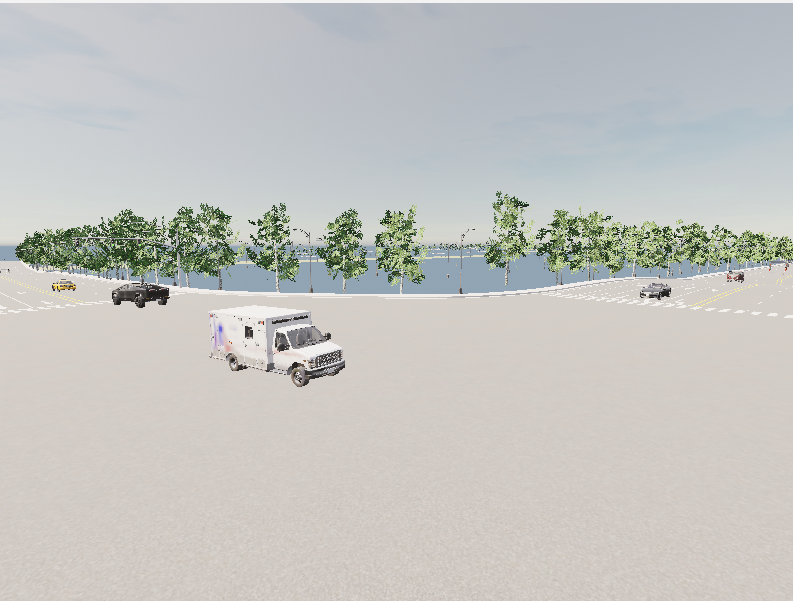
\includegraphics[width=0.75\textwidth]{p44} % 假设图片文件名为car.pdf或car.png等,位于当前工作目录
	\caption{交通流量预测与信号控制的协同优化} % 图片标题
	\label{fig:p44} % 用于引用的标签
\end{figure}




\section{跨摄像头目标再识别与轨迹拼接技术}

\subsection{Re-ID 网络的定制化训练}


构建面向车辆的 Re-ID 网络,基于 ResNet-50 预训练网络获得细粒度的外观 物征(车身颜色、车款),并采用三元组损失来增强判别能力,在 VeRi-776 数据集上 mAP 指标为 85\%,完成跨摄像机视图下的车辆身份匹配。


\subsection{多路口轨迹匹配算法}

提出基于余弦相似度的轨迹拼接方案,提取不同路口的轨迹外观相似度(门限0.65),完成车辆在多个路口之间的轨迹连接,突破以往单一摄像机跟踪的视角限制,形成完整连续的全局车辆轨迹重构系统如图\ref{fig:p45}。


\begin{figure}[htbp] % 可以是h(here),t(top),b(bottom),p(page of floats)
	\centering
	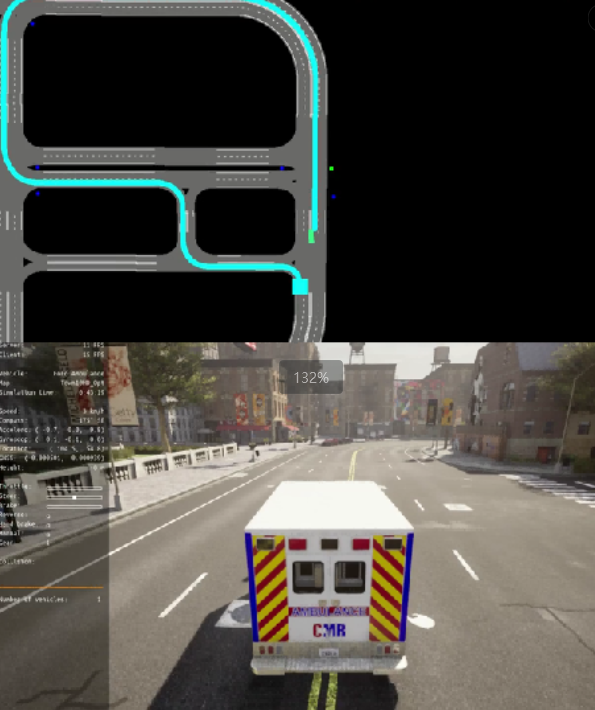
\includegraphics[width=1\textwidth]{p45} % 假设图片文件名为car.pdf或car.png等,位于当前工作目录
	\caption{轨迹拼接} % 图片标题
	\label{fig:p45} % 用于引用的标签
\end{figure}




\section{工程化与实际应用的探索}

\subsection{模块化系统设计}

打造一套“检测-关联-再识别-轨迹重演-精度评价”的闭环系统,子模块(检测、关联、再识别)均可单独训练,可迅速迁移到无人驾驶、路况监控等应用。


\subsection{数字孪生与城市级应用}

设计并基于多目标跟踪的交通数字孪生系统原型,利用车辆轨迹重现技术,可为自动驾驶测试、交通流的优化及应急处理等提供实时的数据信息参考,具有很强的工程意义。


